\documentclass{cup-pan}
\usepackage{blindtext}
\usepackage{siunitx}
\usepackage{float}
\usepackage{ragged2e}
\sisetup{group-separator={,}}
\usepackage{array}
\newcolumntype{P}[1]{>{\centering\arraybackslash}p{#1}}
\usepackage{longtable}

\title{Analysis of Seismic and Tsunami Loads Effects on 10-Story Reinforced Concrete Building based on SNI 1727:2020 with Tsunami Height Variations}

\author[1]{Muhammad Ikhsan}
\author[1]{Ahmad Muhtarom}

\affil[1]{Department Civil Engineering and Planning, Sriwijaya University, Jl. Raya Prabumulih – KM 32, Indralaya, Ogan Ilir, South Sumatera. Email: \url{sipil@ft.unsri.ac.id}}

%% Corresponding author
\corrauthor{Muhammad Ikhsan}
%% Abbreviated author list for the running footer
\runningauthor{Muhammad Ikhsan and Ahmad Muhtarom}

\addbibresource{refs.bib}

\begin{document}

\maketitle

\begin{abstract}
ASCE 7-16 was adopted in Indonesia to become several building codes namely, SNI 1726:2019 for earthquake loads and its requirements and SNI 1727:2020 for minimum loads on buildings. There is a new requirement that differs from SNI 1727:2013 which is tsunami loads. This load is adopted because of its relevance to Indonesia. This study aims to know the structural response of a building subjected to different tsunami heights. Inundation heights varied from one to three floors. Structural acceptance criteria, which include linear acceptance and nonlinear acceptance, were another variation used in this study. Materials specifications, structural topology and loads—with the exception of tsunamis—were fixed variables. Independent variables were tsunami loads and structural acceptance criteria. A comparison was made to deformations, internal forces and structural weights. The results showed that the internal forces due to the tsunami loads occurred as high as the inundation height. The applied tsunami forces were hydrostatic, hydrodynamic and debris impact forces. The hydrodynamic base shear force depends on the height of the tsunami, where the greatest value was in the 3 stories tsunami high, which was \num{38392.68} kN in load case 2. Nonlinear structure acceptance could reduce the bending moment that occurs in the column up to \SI{49.66}{\percent} in comparison with linear structures. The upper floor exterior columns design was generally controlled by debris impact loads whereas the lower floor column was controlled by hydrodynamic loads. The results also show that the 10-story structure is not vulnerable to being lifted by the buoyancy load.



\keywords{Linear Analysis, Nonlinear Analysis, Structural Optimization, Structural Response, Tsunami Loads.}
\end{abstract}

\section{Introduction}
\label{sec:overview}

Extreme natural phenomena such as winds, earthquakes and tsunamis exert lateral loads that can damage structures and even result in loss of life. These incidents are complex and tend to occur regularly, but cannot be predicted with high precision. The ASCE 7 standard (Minimum Design Loads and Associated Criteria for Buildings and Other Structures) quantifies these loads probabilistically based on climatology, geology and seismology from previous data and existing events \citep{leet}.

The ASCE 7 standard with its latest version ASCE 7-16 has been adopted into several standards in Indonesia, including SNI 1726:2019 regarding seismic requirements and SNI 1727:2020 concerning minimum design loads. The tsunami load is a new load that is provided under this new regulation. This load was adopted because it is relevant to Indonesia. The standard will become a new reference for tsunami-prone areas in Indonesia.

Environmental loads in the SNI 1727:2020 consist of vertical loads and also lateral loads. In general, for gravity or vertical loads, there is not much that can be done by engineers to the structure. Many innovations in structural engineering are generally developed to withstand lateral loads that occur in structures \citep{taranath}. The initial design process usually only considers gravity loads, thus additional design processing is required to ensure that the building can withstand the intended lateral loads that are anticipated to be applied to it during the course of its design lifetime.

When an earthquake occurs, the ground suddenly shifts and structures deflect as a result of their inertia, which causes the corresponding lateral load \citep{taranath}. Tsunami and wind loads have almost the same characteristics, which depend on the surface exposed to this force. The tsunami load also has a lifting force that works opposite to the gravitational force, if there is a void that displaces the volume of tsunami water (Archimedes’ principle). These characteristics made earthquake loads to be designed iteratively, while wind and tsunami loads can be designed based on the exposed surface of the building.

The adoption of ASCE 7 standard regarding tsunami load imposed new criteria on buildings in tsunami-prone areas. The tsunami load will certainly add new load cases to the building design. The uplift load on the tsunami load also makes the building must have sufficient weight to prevent lifting from the foundation. The large weight of the building on the other hand also increases the seismic force. This difference in characteristics makes it necessary to conduct research on the effects of tsunami and earthquake loads. In this study, tsunami and earthquake loads will be applied to reinforced concrete structures. Inundation height will be varied to evaluate the response of the reinforced concrete building structure.

\section{Literature review}
\label{sec:litview}

\subsection{Tsunami load}
\label{subsec:tsunami load}

The tsunami consists of several wave stages, which are simplified to three load cases in the tsunami loading. ASCE and SNI provide a simple relationship between inundation depth and inflow and outflow velocity. Load cases 2 and 3 represent the critical combination of water level and flow velocity that occurs during the tsunami.

Load case 2 considers the maximum velocity, $u_{max}$, during inflow and outflow when the inundation depth is $\frac{2}{3}$ of, $h_{max}$, the largest inundation depth during the tsunami. It produces the largest hydrodynamic forces. When applied to stationary objects, water velocity produces hydrodynamic forces (in this case nonmoving structures).

Load case 3 represents the loading due to the maximum inundation depth, $h_{max}$, and a flow velocity as large as $\frac{1}{3}$ of the maximum flow velocity, $u_{max}$. This load case produces the force due to the largest inundation height, therefore the largest exposed surface of the building. It is meant to load all possible structural elements during the tsunami.

Load case 1 assumes the inundation height which produces the greatest buoyancy forces together with the hydrodynamic forces which have velocity corresponding to the inundation height. The summary of load cases in tsunami loading according to ASCE 7-16 and SNI 1727:2020 can be found in table \ref{tab:tsunami load cases}. The inflow and outflow height of inundation and the corresponding velocity is also illustrated in figure \ref{fig:loadcases}.

%\begin{table}[H]
%\renewcommand{\arraystretch}{1.5}

%\centering

\renewcommand{\arraystretch}{1}
\begin{longtable}{P{1in} P{1in} P{1in} P{1.5in}}
\caption{Summary of tsunami load cases according to ASCE 7-16 and SNI 1727:2020. Source: \cite{leet}.}\\

\headrow \thead{Load Case} & \thead{h\textsubscript{des}} & \thead{u\textsubscript{des}} & \thead{Load implication} \\
1& $h$ which causes maximum buoyancy forces     & $u$ which coressponds to $h$ & Maximum uplift forces \\
2& $\frac{2}{3}h_{max}$     & $u_{max}$       & Maximum hydrodynamic loads         \\
3     & $h_{max}$      &   $\frac{1}{3}u_{max}$            & Maximum numbers of structural elements to be loaded  \\
\label{tab:tsunami load cases}
\end{longtable}
%\end{table}  

The tsunami load under consideration must be determined by the graph in figure \ref{fig:loadcases} which shows the relationship between the inundation depth ratio and the velocity ratio for each load case.

\begin{figure}[H]
\centering
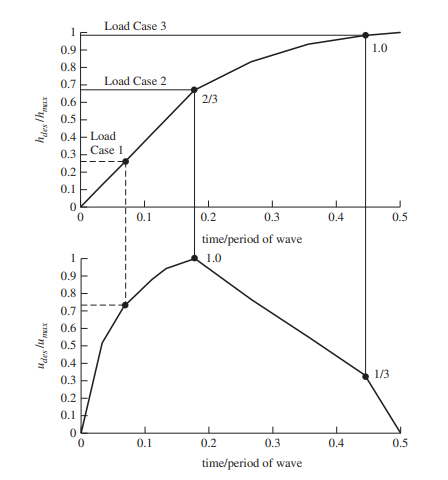
\includegraphics[width=0.6\textwidth]{fig1.png}
\caption{The relationship between inundation height and flow velocity for three cases of tsunami loading \citep{leet}.}
\label{fig:loadcases}
\end{figure}

\subsubsection{Hydrostatic load}

\section{Methodology}
\label{sec:method}

The following is the research flowchart used in this study:

\section{Results and discussion}
\label{sec:results}

Earthquakes model structural design was carried out by using heuristic optimization. Design optimization is done by adjusting the member sizes to the behavior of the structure. The structural member size results to resist earthquake load according to the Banda Aceh spectrum response with soft soil conditions are given in figures \ref{fig:XZ view} and \ref{fig:YZ view}.

\begin{figure}[H]
\centering
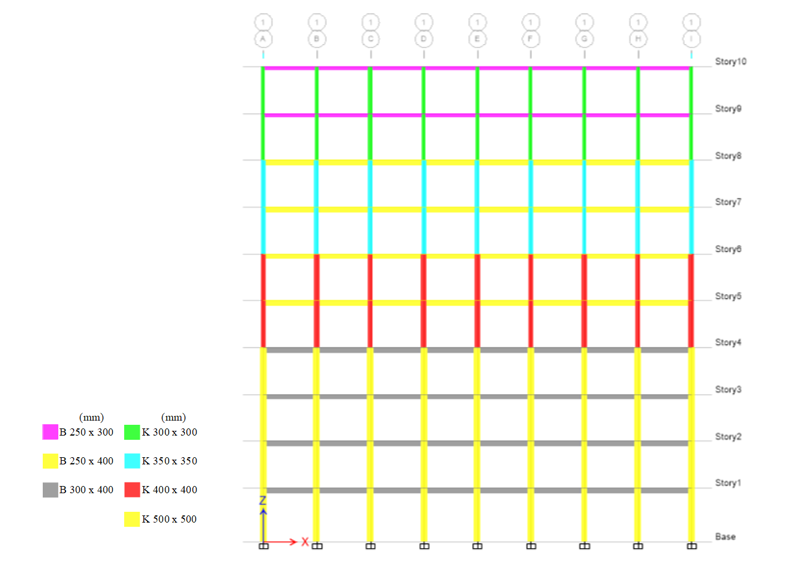
\includegraphics[width=0.6\textwidth]{Picture6.png}
\caption{XZ elevation view of the design result.}
\label{fig:XZ view}
\end{figure}

\begin{figure}[H]
\centering
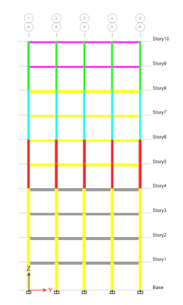
\includegraphics[width=0.3\textwidth]{Picture7.png}
\caption{YZ elevation view of the design result.}
\label{fig:YZ view}
\end{figure}

The structure was designed to have typical beams and columns for one floor. A summary of the cross-section of the building per floor can be seen in table \ref{tab:cross section model 1}. The building has a structural weight of, $W_{structure}=\num{27652,93} \si{kN}$. The base shear force for the seismic load in Banda Aceh for that particular structure was, $E_h=\num{2988,62} \si{kN}$.

%\begin{table}[H]
\renewcommand{\arraystretch}{1}
%\centering
\begin{longtable}{P{0.75in} P{1.25in} P{1.25in} P{1.25in}}
\caption{Summary of structural elements in model 1 (earthquake loads only).}\\
\headrow \thead{Floor} & \thead{Beam cross section (mm)} & \thead{Column cross section (mm)} & \thead{Structure weight (kN)} \\
1 & $300 \times 400$ & $500 \times 500$ & \num{3256.43}  \\
2 & $300 \times 400$ & $500 \times 500$ & \num{3124.04}  \\
3 & $300 \times 400$ & $500 \times 500$ & \num{3124.04}  \\
4 & $300 \times 400$ & $500 \times 500$ & \num{3124.04}  \\
5 & $250 \times 400$ & $400 \times 400$ & \num{2683.10}  \\
6 & $250 \times 400$ & $400 \times 400$ & \num{2683.10}  \\
7 & $250 \times 400$ & $350 \times 350$ & \num{2553.03}  \\
8 & $250 \times 400$ & $350 \times 350$ & \num{2553.03}  \\
9 & $250 \times 300$ & $300 \times 300$ & \num{2276.04}  \\
10 & $250 \times 300$ & $300 \times 300$ & \num{2276.04}  \\
 &  & Total structural weight & \num{27652.93}  \\
\label{tab:cross section model 1}
\end{longtable}
%\end{table}  

Drifts evaluation were performed for seismic forces with and without induced torsion for each of the direction. The induced torque is given from an eccentricity of \SI{5}{\percent} of the size of the diaphragm perpendicular to the seismic force for each direction. The drift calculation results for each load case are presented in figure \ref{fig:driftchecking}.

\begin{figure}[H]
\centering
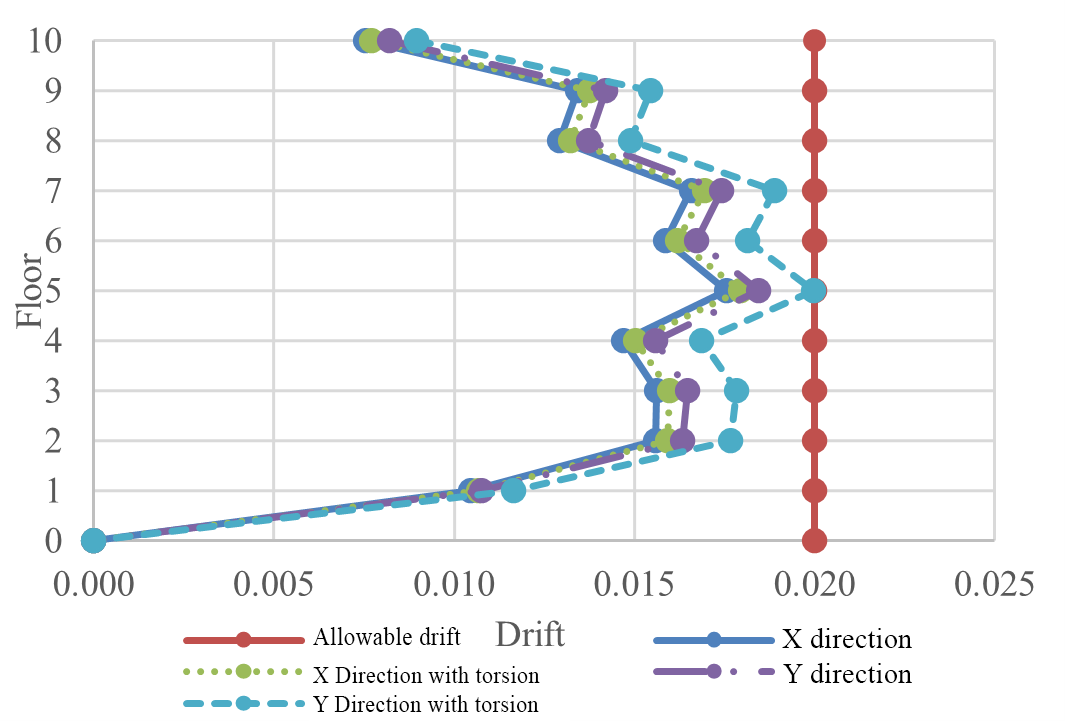
\includegraphics[width=0.7\textwidth]{Picture8_engels.png}
\caption{Drift checking in earthquake model (model 1).}
\label{fig:driftchecking}
\end{figure}

Structures that were built to withstand seismic forces had their designs tested for tsunami loading. A summary of the tsunami force calculations for load cases 1, 2 and 3 in accordance with figure \ref{fig:loadcases} can be seen in figures \ref{fig:lc1}, \ref{fig:lc2} and \ref{fig:lc3}. These loads were applied to each floor.

\begin{figure}[H]
\centering
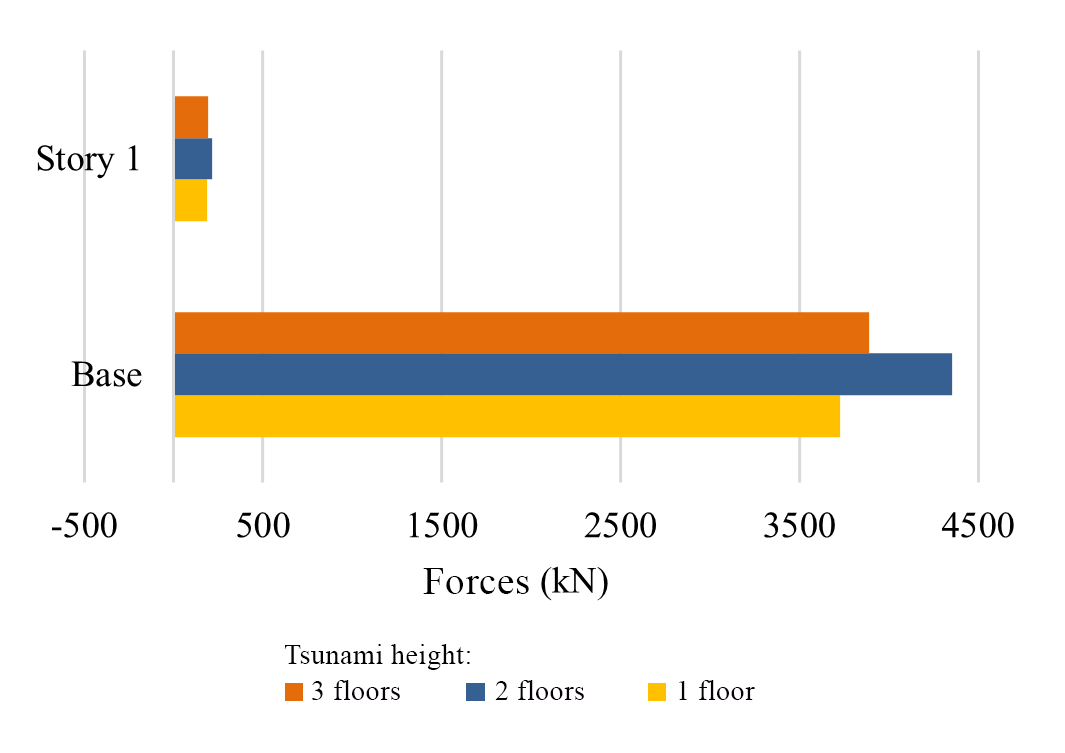
\includegraphics[width=0.5\textwidth]{Picture9_engels.png}
\caption{Tsunami forces for load case 1.}
\label{fig:lc1}
\end{figure}

\begin{figure}[H]
\centering
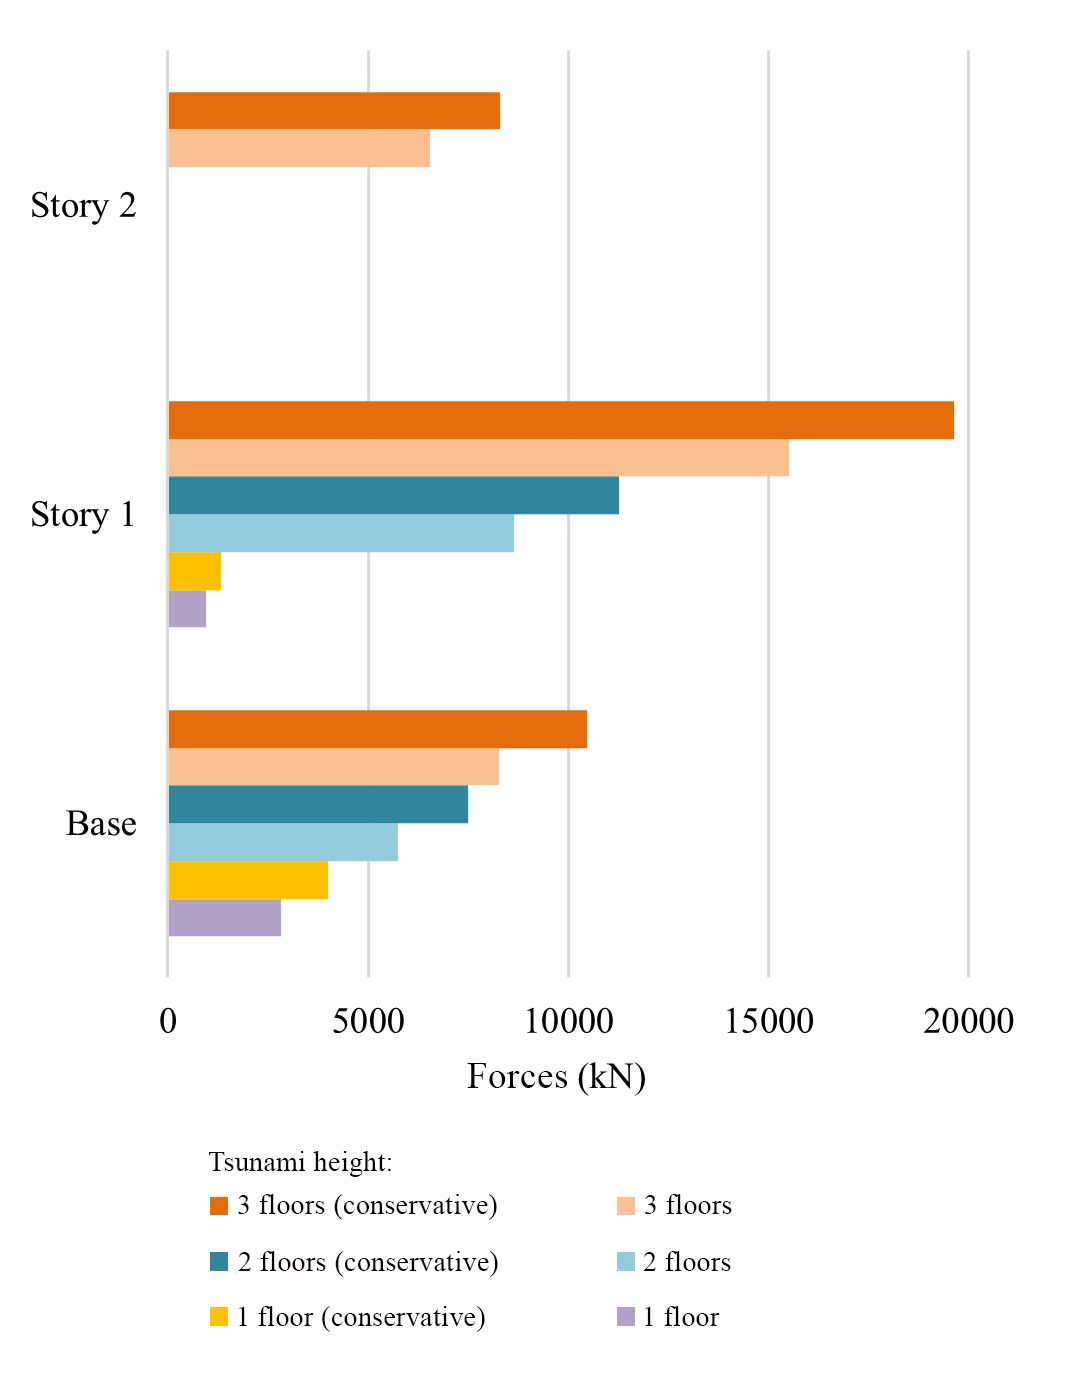
\includegraphics[width=0.5\textwidth]{Picture10_engels.png}
\caption{Tsunami forces for load case 2.}
\label{fig:lc2}
\end{figure}

\begin{figure}[H]
\centering
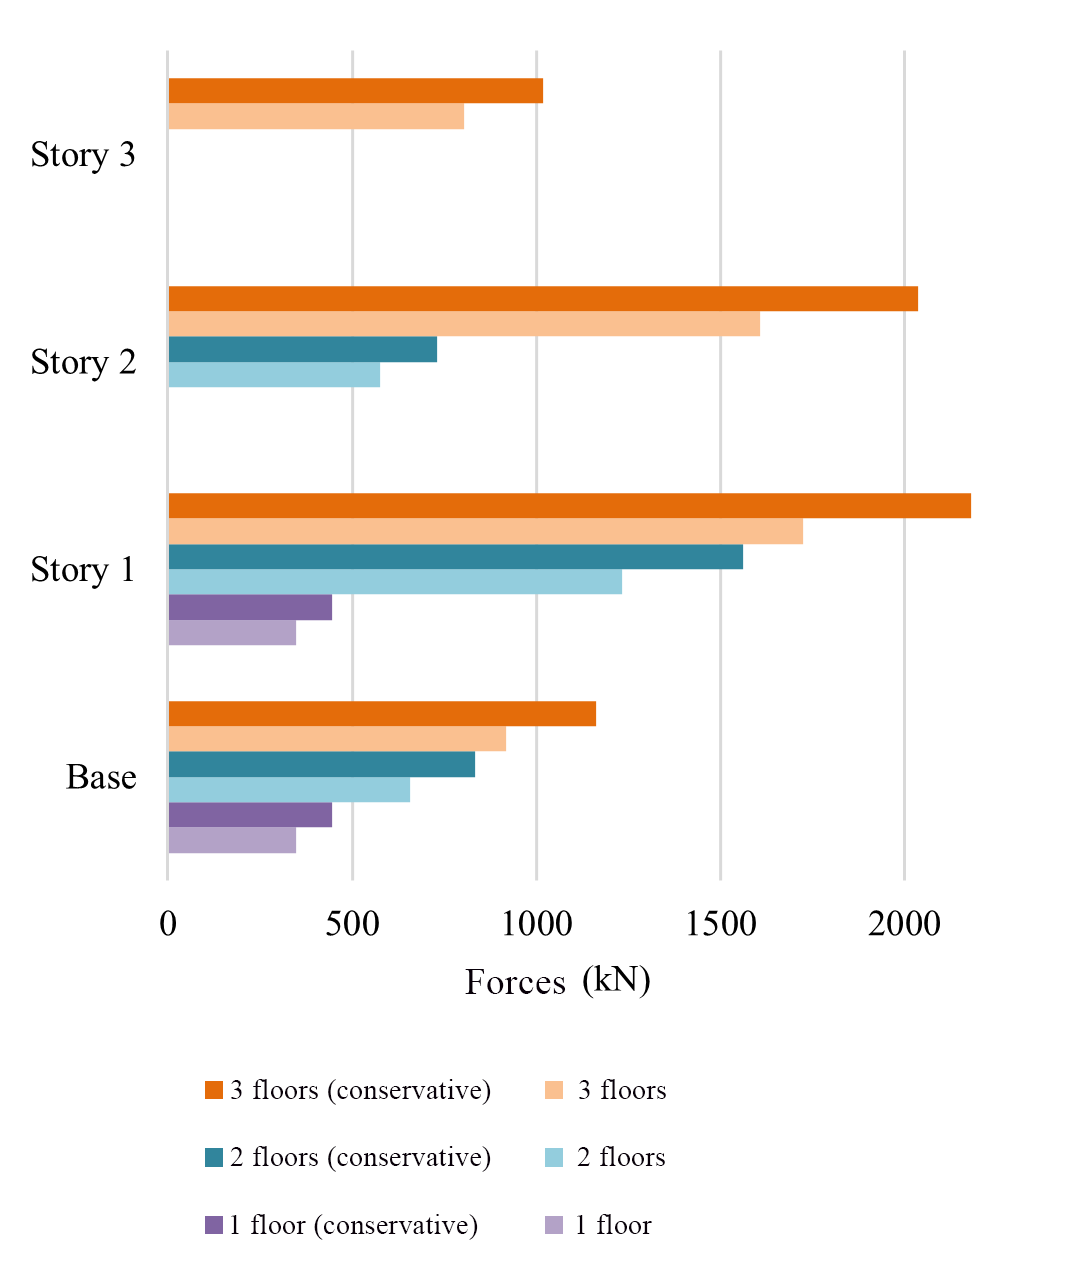
\includegraphics[width=0.5\textwidth]{Picture11_engels.png}
\caption{Tsunami forces for load case 3.}
\label{fig:lc3}
\end{figure}

The structure of model 1, in table \ref{tab:cross section model 1} was loaded with each load case within each model and optimized to resist the loads with the corresponding structural acceptance criteria according to table \ref{tab:model definition}. The results of structural optimization for each tsunami load model can be seen from table \ref{tab:cross section model 2} to \ref{tab:cross section model 7}.

\renewcommand{\arraystretch}{1}
\begin{longtable}{P{0.5in} P{1in} P{1in} P{1in} P{1in}}
\caption{Summary of structural elements in model 2.}\\
\headrow \thead{Floor} & \thead{Interior column (mm)} & \thead{Exterior column (mm)} & \thead{Beam (mm)} & \thead{Structure weight (kN)} \\
1 & $500 \times 500$ & $600 \times 600$ & $300 \times 400$ & \num{3495.37} \\
2 & $500 \times 500$ & $500 \times 500$ & $300 \times 400$ & \num{3124.04} \\
3 & $500 \times 500$ & $500 \times 500$ & $300 \times 400$ & \num{3124.04} \\
4 & $500 \times 500$ & $500 \times 500$ & $300 \times 400$ & \num{3124.04} \\
5 & $400 \times 400$ & $400 \times 400$ & $250 \times 400$ & \num{2683.10} \\
6 & $400 \times 400$ & $400 \times 400$ & $250 \times 400$ & \num{2683.10} \\
7 & $350 \times 350$ & $350 \times 350$ & $250 \times 400$ & \num{2553.03} \\
8 & $350 \times 350$ & $350 \times 350$ & $250 \times 400$ & \num{2553.03} \\
9 & $300 \times 300$ & $300 \times 300$ & $250 \times 300$ & \num{2276.04} \\
10 & $300 \times 300$ & $300 \times 300$ & $250 \times 300$ & \num{2276.04} \\
 &  & & Total structural weight & \num{27891.86} \\
\label{tab:cross section model 2}
\end{longtable}

\renewcommand{\arraystretch}{1}
\begin{longtable}{P{0.5in} P{1in} P{1in} P{1in} P{1in}}
\caption{Summary of structural elements in model 3.} \\
\headrow \thead{Floor} & \thead{Interior column (mm)} & \thead{Exterior column (mm)} & \thead{Beam (mm)} & \thead{Structure weight (kN)} \\
1 & $500 \times 500$ & $550 \times 550$ & $300 \times 400$ & \num{3370.25} \\
2 & $500 \times 500$ & $500 \times 500$ & $300 \times 400$ & \num{3124.04} \\
3 & $500 \times 500$ & $500 \times 500$ & $300 \times 400$ & \num{3124.04} \\
4 & $500 \times 500$ & $500 \times 500$ & $300 \times 400$ & \num{3124.04} \\
5 & $400 \times 400$ & $400 \times 400$ & $250 \times 400$ & \num{2683.10} \\
6 & $400 \times 400$ & $400 \times 400$ & $250 \times 400$ & \num{2683.10} \\
7 & $350 \times 350$ & $350 \times 350$ & $250 \times 400$ & \num{2553.03} \\
8 & $350 \times 350$ & $350 \times 350$ & $250 \times 400$ & \num{2553.03} \\
9 & $300 \times 300$ & $300 \times 300$ & $250 \times 300$ & \num{2276.04} \\
10 & $300 \times 300$ & $300 \times 300$ & $250 \times 300$ & \num{2276.04} \\
 &  & & Total structural weight & \num{27766.74} \\
\label{tab:cross section model 3}
\end{longtable}

\renewcommand{\arraystretch}{1}
\begin{longtable}{P{0.5in} P{1in} P{1in} P{1in} P{1in}}
\caption{Summary of structural elements in model 4.}\\
\headrow \thead{Floor} & \thead{Interior column (mm)} & \thead{Exterior column (mm)} & \thead{Beam (mm)} & \thead{Structure weight (kN)} \\
1 & $650 \times 650$ & $1000 \times 1000$ & $350 \times 500$ & \num{5540.42} \\
2 & $500 \times 500$ & $550 \times 550$ & $300 \times 400$ & \num{3223.03} \\
3 & $500 \times 500$ & $500 \times 500$ & $300 \times 400$ & \num{3124.04} \\
4 & $500 \times 500$ & $500 \times 500$ & $300 \times 400$ & \num{3124.04} \\
5 & $400 \times 400$ & $400 \times 400$ & $250 \times 400$ & \num{2683.10} \\
6 & $400 \times 400$ & $400 \times 400$ & $250 \times 400$ & \num{2683.10} \\
7 & $350 \times 350$ & $350 \times 350$ & $250 \times 400$ & \num{2553.03} \\
8 & $350 \times 350$ & $350 \times 350$ & $250 \times 400$ & \num{2553.03} \\
9 & $300 \times 300$ & $300 \times 300$ & $250 \times 300$ & \num{2276.04} \\
10 & $300 \times 300$ & $300 \times 300$ & $250 \times 300$ & \num{2276.04} \\
 &  & & Total structural weight & \num{30035.91} \\
\label{tab:cross section model 4}
\end{longtable}

\renewcommand{\arraystretch}{1}
\begin{longtable}{P{0.5in} P{1in} P{1in} P{1in} P{1in}}
\caption{Summary of structural elements in model 5.}\\
\headrow \thead{Floor} & \thead{Interior column (mm)} & \thead{Exterior column (mm)} & \thead{Beam (mm)} & \thead{Structure weight (kN)} \\
1 & $650 \times 650$ & $650 \times 650$ & $300 \times 400$ & \num{3124.04} \\
2 & $500 \times 500$ & $550 \times 550$ & $300 \times 400$ & \num{3223.03} \\
3 & $500 \times 500$ & $500 \times 500$ & $300 \times 400$ & \num{3124.04} \\
4 & $500 \times 500$ & $500 \times 500$ & $300 \times 400$ & \num{3124.04} \\
5 & $400 \times 400$ & $400 \times 400$ & $250 \times 400$ & \num{2683.10} \\
6 & $400 \times 400$ & $400 \times 400$ & $250 \times 400$ & \num{2683.10} \\
7 & $350 \times 350$ & $350 \times 350$ & $250 \times 400$ & \num{2553.03} \\
8 & $350 \times 350$ & $350 \times 350$ & $250 \times 400$ & \num{2553.03} \\
9 & $300 \times 300$ & $300 \times 300$ & $250 \times 300$ & \num{2276.04} \\
10 & $300 \times 300$ & $300 \times 300$ & $250 \times 300$ & \num{2276.04} \\
 &  & & Total structural weight & \num{28450.52} \\
\label{tab:cross section model 5}
\end{longtable}

\renewcommand{\arraystretch}{1}
\begin{longtable}{P{0.5in} P{1in} P{1in} P{1in} P{1in}}
\caption{Summary of structural elements in model 6.}\\
\headrow \thead{Floor} & \thead{Interior column (mm)} & \thead{Exterior column (mm)} & \thead{Beam (mm)} & \thead{Structure weight (kN)} \\
1 & $900\times900$ & $900\times1400$ & $400\times600$ & \num{7182.79} \\
2 & $800\times800$ & $800\times800$ & $400\times600$ & \num{5192.22} \\
3 & $500\times500$ & $550\times550$ & $300\times400$ & \num{3223.03} \\
4 & $500\times500$ & $500\times500$ & $300\times400$ & \num{3124.04} \\
5 & $400\times400$ & $400\times400$ & $250\times400$ & \num{2683.10} \\
6 & $400\times400$ & $400\times400$ & $250\times400$ & \num{2683.10} \\
7 & $350\times350$ & $350\times350$ & $250\times400$ & \num{2553.03} \\
8 & $350\times350$ & $350\times350$ & $250\times400$ & \num{2553.03} \\
9 & $300\times300$ & $300\times300$ & $250\times300$ & \num{2276.04} \\
10 & $300\times300$ & $300\times300$ & $250\times300$ & \num{2276.04} \\
 &  & & Total structural weight & \num{33746.46} \\
\label{tab:cross section model 6}
\end{longtable}

\renewcommand{\arraystretch}{1}
\begin{longtable}{P{0.5in} P{1in} P{1in} P{1in} P{1in}}
\caption{Summary of structural elements in model 7.}\\
\headrow \thead{Floor} & \thead{Interior column (mm)} & \thead{Exterior column (mm)} & \thead{Beam (mm)} & \thead{Structure weight (kN)} \\
1 & $900\times900$ & $900\times900$ & $300\times400$ & \num{5543.00} \\
2 & $700\times700$ & $700\times700$ & $300\times400$ & \num{3970.77} \\
3 & $500\times500$ & $550\times550$ & $300\times400$ & \num{3223.03} \\
4 & $500\times500$ & $500\times500$ & $300\times400$ & \num{3124.04} \\
5 & $400\times400$ & $400\times400$ & $250\times400$ & \num{2683.10} \\
6 & $400\times400$ & $400\times400$ & $250\times400$ & \num{2683.10} \\
7 & $350\times350$ & $350\times350$ & $250\times400$ & \num{2553.03} \\
8 & $350\times350$ & $350\times350$ & $250\times400$ & \num{2553.03} \\
9 & $300\times300$ & $300\times300$ & $250\times300$ & \num{2276.04} \\
10 & $300\times300$ & $300\times300$ & $250\times300$ & \num{2276.04} \\
 &  & & Total structural weight & \num{30885.21} \\
\label{tab:cross section model 7}
\end{longtable}

In Figure \ref{fig:base shear} it can be seen that for models 2 and 3 the tsunami base shear force that occurs was smaller than the seismic base shear force with an overstrength factor. This was consistent with the results of structural analysis, where the dimensional changes in the exterior columns were only caused by local forces which were the debris impact loads. The moment resisting system for models 2 and 3 did not need to be changed from model 1 to withstand a tsunami load as high as 1 floor. Changes were made due to local tsunami loads in the form of local hydrodynamic forces and debris impact loads. In model 4 the tsunami base shear force that occurs exceeds the capacity resulting from the seismic base shear force with an overstrength factor, thus it was necessary to change the dimensions of the lateral force resisting systems.

\begin{figure}[H]
\centering
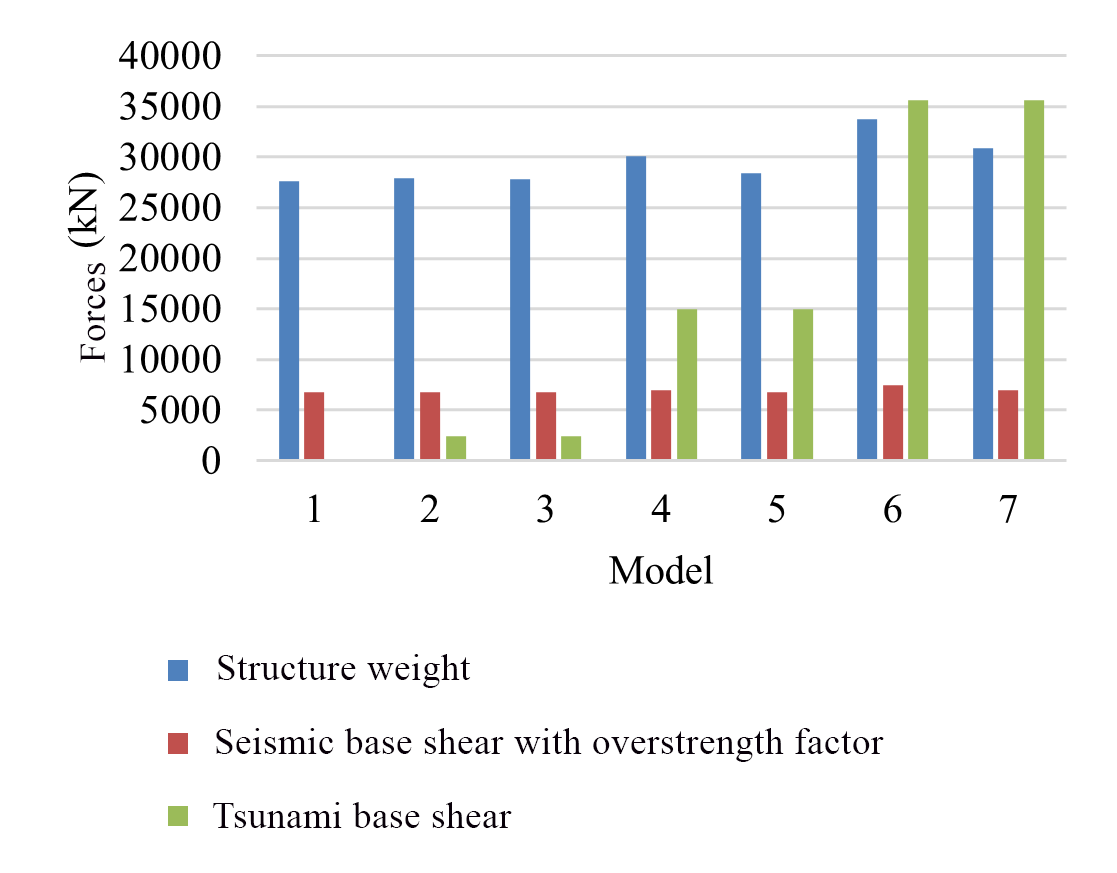
\includegraphics[width=0.7\textwidth]{Picture12_engels.png}
\caption{Structural weight and base shear forces.}
\label{fig:base shear}
\end{figure}

The maximum forces in beams and columns were compared for each model. The forces for the beam elements were reviewed for the case of the overall hydrodynamic load. The internal force for the beam elements was taken for the largest value for each model, for support and middle section values. Figures \ref{fig:maxmomentbeam} and \ref{fig:maxshearbeam} show the maximum values for internal forces in each model for beam structural elements.

\begin{figure}[H]
\centering
\includegraphics[width=0.6\textwidth]{Picture13_engels.png}
\caption{Maximum bending moment for beams in each model.}
\label{fig:maxmomentbeam}
\end{figure}

\begin{figure}[H]
\centering
\includegraphics[width=0.6\textwidth]{Picture14_engels.png}
\caption{Maximum shear force for beams in each model.}
\label{fig:maxshearbeam}
\end{figure}


The internal forces for the columns were taken in the case of component hydrodynamic loads for the exterior and interior columns. The internal forces taken were in the form of axial force, shear force and bending moment. The internal forces taken were for the exterior column and interior column. Figures \ref{fig:maxaxialcolumn} to \ref{fig:maxmomentcolumn} show the plot of internal forces for column structural elements for each model.

\begin{figure}[H]
\centering
\includegraphics[width=0.6\textwidth]{Picture15_engels.png}
\caption{Maximum axial force for columns in each model.}
\label{fig:maxaxialcolumn}
\end{figure}

\begin{figure}[H]
\centering
\includegraphics[width=0.6\textwidth]{Picture16_engels.png}
\caption{Maximum shear force for columns in each model.}
\label{fig:maxshearcolumn}
\end{figure}

\begin{figure}[H]
\centering
\includegraphics[width=0.6\textwidth]{Picture17_engels.png}
\caption{Maximum bending moment for columns in each model.}
\label{fig:maxmomentcolumn}
\end{figure}


\renewcommand{\arraystretch}{1}
\begin{longtable}{P{0.5in} P{1in} P{1in} P{1in} P{1in}}
\caption{Summary of critical axial forces in base columns to determine lifting.}\\
\headrow \thead{Model} & \thead{Interior column (kN)} & \thead{Middle exterior column (kN)} & \thead{Corner exterior column (kN)} & \thead{Conclusion} \\
2 & $-504.07$ & $-618.97$ & $-528.01$ & No lifting occured \\
3 & $-501.67$ & $-622.72$ & $-534.52$ & No lifting occured \\
4 & $-262.26$ & $-497.11$ & $-460.46$ & No lifting occured \\
5 & $-155.76$ & $-428.88$ & $-416.76$ & No lifting occured \\
6 & $-321.36$ & $-399.90$ & $-345.58$ & No lifting occured \\
7 & $-344.96$ & $-387.64$ & $-360.95$ & No lifting occured \\
\label{tab:recap lifting}
\end{longtable}

\section{Conclusion}
\label{sec:conclusion}
\begin{enumerate}
\item{The internal forces due to the earthquake had a comparable magnitude to the force in the beam due to the tsunami loads. The forces in the beam due to the earthquake were exceeded in a 3-story high tsunami. For example, the support bending moment of model 1 (earthquake only) had a magnitude of \num{-80.56} \si{kN.m} for negative bending moments, this value had only been exceeded in model 6 which had a value of \num{-123.60} \si{kN.m}. Meanwhile, internal forces in the column had a magnitude that far exceeds the internal forces due to the earthquake loads, especially for shear forces and bending moments. Acceptance of the structure in models 2 to 7 also affects the internal forces that occur. Acceptance of nonlinear models can reduce the bending moment that occurs in the column up to \SI{49.66}{\percent} compared to the linear models.}

\item{The lifting force that occurred had not been able to lift the structure as a whole. The most significant net force was \num{155.76} \si{kN} (downward). This smallest net force occurred in the interior column of model 5 (2-story tsunami with nonlinear acceptance criteria). This indicated that the weight of the structure was able to counteract the lifting force that occurred.}

\item{The inundation height has an effect on the hydrodynamic force. The higher the tsunami, the greater the hydrodynamic force. The magnitude of the tsunami base shear force on the models with inundation height of 1 floor, 2 floors and 3 floors respectively were \num{2400.64} \si{kN}; \num{15003.99} \si{kN}; \num{35600.49} \si{kN}. The increase in the base shear force occurs exponentially because the magnitude of the force depends on the square of the velocity with the upper limit of \num{15.20} \si{m/s}. The maximum bending moment that occurs in the exterior column on the models with tsunami as height as 1 floor, 2 floors and 3 floors respectively were \num{680.52} \si{kN.m}; \num{3086.75} \si{kN.m}; and \num{6629.72} \si{kN.m}. These internal forces increase significantly in relation to the tsunami height of each model.
}

\item{The tsunami load affects the design of structural elements up to the tsunami height. Structural elements that are above the inundation level are generally not affected by the tsunami that occurs. The upper-floor exterior columns were generally controlled by debris impact loads. The lower-column were controlled by hydrodynamic loads. The weight of all models differs from the earthquake model (model 1). The largest structural weight was in model 6 (3-floor tsunami with linear acceptance criteria) which was \num{33746.46} \si{kN} or an increase of \SI{22.03}{\percent} from model 1.}
\end{enumerate}

Only two levels of sectional headings, \verb|\section| and \verb|\subsection|, should be used. Ad nemo aut quae dolores nesciunt reprehenderit occaecati. Optio distinctio at aliquam odit dolores laudantium. Illum et qui iste et laudantium dolorum. Nihil quis qui at quia alias. Quisquam ea sit aspernatur. Labore at hic voluptas cumque eum officia repellat.

Here's an example parenthetical citation \citep{asce} and a text citation: \citet{asce}. There isn't a good, up-to-date BibTeX style for the Chicago style, so we're using \texttt{biblatex-chicago} instead. This means you'll need to run \texttt{biber} instead of \texttt{bibtex} if you're compiling this template on your local \LaTeX{} installation: on Overleaf, \texttt{biber} is run automatically. You can add pre-notes with citations \citep[see also][]{asce} too, as well as multiple citations \citep{asce,asce} in a single \verb|\citep{...}| or \verb|\citet{...}|. 

This is an equation, numbered
\begin{equation}
l(\Lambda)=\sum_{i=1}^{n} \sum_{w=1}^{q} (z_{i w} \ln (\lambda_{i w}) - \lambda_{i w} - \ln (z_{i w}!))
\label{eq:poisson}
\end{equation}
and one that is not numbered
\begin{equation*}
\int_0^{+\infty}e^{-x^2}dx=\frac{\sqrt{\pi}}{2}
\end{equation*}
and one inlined: $e^{i\pi}=-1$. As usual you can cross-reference equations with Equation \ref{eq:poisson} or \eqref{eq:poisson}.

Figure \ref{fig:example} shows a normal figure, while figure \ref{fig:twosubs} show one made up of two sub-figures. Figure \ref{fig:landscape} is an example of a landscaped figure. You can use the \verb|\subcaption{...}| command from the \texttt{subcaption} package to add captions for subfigures and subtables, but do not use the \texttt{subfigure} package: it is incompatible with this template.


\begin{figure}
\begin{minipage}{0.47\textwidth}
\includegraphics[width=\linewidth]{example-image}
\subcaption{This is a subfigure}
\end{minipage}
\hfill
\begin{minipage}{0.47\textwidth}
\includegraphics[width=\linewidth]{example-image}
\subcaption{This is another subfigure}
\end{minipage}

\caption{This is a caption for the entire figure}
\label{fig:twosubs}
\end{figure}

\begin{sidewaysfigure}
\centering
\includegraphics[width=19cm]{example-image}
\caption{This is a figure caption}
\label{fig:landscape}
\end{sidewaysfigure}

\blinddocument

\bigskip

\paragraph*{Acknowledgments.} We are grateful for the technical assistance of A.~Author.

\paragraph*{Data Availability Statement.} Replication data and code can be found in Harvard Dataverse: \url{https://doi.org/link}.

\nocite{*}
\printbibliography
\end{document}
